\chapter{Implementacja}

\section{Architektura}


\subsection{Struktura interfejsu REST}
% TO DO: Opis do poprawy (bo zmieniono układ tabel)
% DONE
Tabele \ref{tab:rest1} oraz \ref{tab:rest2} prezentują jakie zapytania mogą być odbierane przez aplikację serwerową. Z racji tego, że w aplikacji wykorzystywane są typy generyczne w klasach kontrolerach urządzeń i komponentów komputera (implementacja \ref{controller_genericDevice} uproszczono tabele by pokazać ogólną formę zapytań. Wszystkie zapytania posiadające "`\texttt{devices}"' w ścieżce umożliwiają alternatywne wywołanie zapytania na podstawie typu sprzętu. Ogólna zasada jest taka aby zastąpić "`\texttt{devices}"' odpowiadającemu typowi sprzętu: "`\texttt{computers}"', "`\texttt{tablets}"', "`\texttt{other-devices}"'. Powoduje to, że zapytanie wykonywane jest przez kontroler tej klasy, a co za tym idzie ma określony typ. Możliwe jest też wykonanie zapytania nie zmieniając ścieżki. Wtedy takie zapytanie wykonywane jest na ogólnym rodzaju sprzętu. Przykładowo "`\texttt{devices/all}"' pobiera wszystkie sprzęty nie zwracając uwagi na typ, natomiast "`\texttt{computers/all}"' pobiera tylko sprzętu typu "`\texttt{Computer}"'. Podobne rozwiązanie wykorzystano w komponentach komputera. Dotyczy to zapytań mających w ścieżce: "`\texttt{component}"'. Tutaj należy zamienić "`\texttt{component}"' na jeden z trzech dostępnych typów komponentu: "`\texttt{rams}"', "`\texttt{cpus}"', "`\texttt{storages}"'. W tym wypadku nie ma możliwości wywołania zapytania zawierającego "`\texttt{component}"'.

\begin{table}[H]\small
	\centering
\caption{Tabela prezentująca strukturę REST (cz.1)}
\label{tab:rest1}
\begin{tabularx}{\linewidth}{|X|l|p{3cm}|X|}
    \hline
    Ścieżka & Metoda & Parametry & Opis  \\
    \hline \hline
		/devices/all 	& GET & - & Pobranie danych sprzętów na podstawie określonego typu \\
		\hline
		/devices/{id} & GET & id urządzenia 	& Pobranie danych wszystkich sprzętów\\
    \hline
		/devices/{id}	& DELETE & id urządzenia 	& Usunięcie sprzętu\\
    \hline
		 /computers/update/id & PATCH & id sprzętu oraz zmienione dane sprzętu& aktualizacja danych komputera\\
		\hline
		 /tablets/update/id & PATCH & id sprzętu oraz zmienione dane sprzętu& aktualizacja danych tabletu\\
		\hline	 
		/other-device/update/id & PATCH & id sprzętu i zmienione dane sprzętu & aktualizacja danych innego urządzenia\\
		\hline
			 /computers/add & POST	& dane komputera 	& Dodanie nowego komputera	\\
    \hline
		/tablets/add & POST	& dane tabletu & Dodanie nowego urządzenia	\\
    \hline
		/other-device/add & POST	& dane innego urządzenia 	& Dodanie nowego urządzenia	\\
    \hline
		/devices/by-office& GET	& id biura 	& Pobranie danych sprzętu znajdujących się w biurze\\
    \hline
		/devices/all-ready-to-lottery& GET	& - & Pobranie danych sprzętów które są gotowe do losowania\\
    \hline
		
		/devices/all-ready-to-lottery-by-officeId/id& GET	& id biura & Pobranie danych sprzętów które są gotowe do losowania i znajdują się w danym biurze\\
    \hline
		/devices/set-ready-to-lottery/id 		& PUT	& id sprzętu & Ustawienie gotowości sprzętu do losowania	\\
    \hline
		/devices/set-not-ready-to-lottery/id & PUT	& id sprzętu & Ustawienie braku gotowości sprzętu do losowania	\\
    \hline
		/devices/set-ordered/id & PUT	& id sprzętu & Ustawienie statusu sprzętu na dostarczone	do pracownika	\\
    \hline
		/devices/set-not-ordered/id & PUT	& id sprzętu & Ustawienie statusu sprzętu na dostarczone	do pracownika	\\
    \hline
		/components/all 	& GET & - & Pobranie danych wszystkich procesorów, ram lub dysków pamięci \\
		\hline
		/components/{id} & GET & id komponentu 	& Pobranie danych procesora, ram lub dysku pamięci\\
    \hline
		/components/{id}	& DELETE & id komponentu 	& Usunięcie procesora, ram lub dysku pamięci\\
    \hline
		 /components/update/id & PUT & id sprzętu oraz zmienione dane sprzętu& aktualizacja danych komputera\\
		\hline
		 /offices/all	& GET & - & Pobranie wszystkich biur w systemie\\
		\hline
		/users/all	& GET & - & Pobranie wszystkich użytkowników w systemie\\
		\hline
		\end{tabularx}
		\end{table}

\begin{table}[H] \small
	\centering
\caption{Tabela prezentująca strukturę REST (cz.2)}
\label{tab:rest2}	 
\begin{tabularx}{\linewidth}{|X|l|p{3cm}|X|}\hline
    Ścieżka & Metoda & Parametry & Opis  \\
    \hline \hline
		 /users/all-standard	& GET & -& Pobranie wszystkich użytkowników z rolą pracownik w systemie\\
		\hline
		 /users/id & GET & - & Pobranie użytkownika\\
		\hline
		 /users/id & DELETE & - & Usunięcie użytkownika\\
		\hline
		 /participation/add & POST & id użytkownika oraz id urządzenia & Dodanie uczestnictwa użytkownika w loterii do wybranego sprzętu\\
		\hline
		 /participation/all& POST & - & Wyświetlenie wszystkich uczestników dla każdego sprzętu\\
		\hline
		 /participation/id & DELETE & - & Usunięcie uczestnictwa o zadanym id\\
		\hline
		 /participation/delete-by-user\_id-and-device\_id& DELETE & id użytkownika i id sprzętu & Usunięcie uczestnictwa spełniającego zadane kryteria\\
		\hline
		 /participation/all-wins& GET & - & Wyświetlenie wszystkich zwycięskich uczestników\\
		\hline
		 /participation/user-lottery-history/id & GET& id użytkownika & Wyświetlenie historii uczestnictwa użytkownika o zadanym id\\
		\hline
		 /participation/user-win-history/id & GET& id użytkownika & Wyświetlenie historii zwycięstw użytkownika o zadanym id\\
		\hline
		 /participation/user-lose-history/id & GET& id użytkownika & Wyświetlenie historii porażek użytkownika o zadanym id\\
		\hline
		 /participation/user-pending-lottery/id & GET& id użytkownika & Wyświetlenie uczestnictwa które czeka na losowanie\\
		\hline
		 /participation/device-participation/id& GET& id urządzenia & Wyświetlenie wszystkich użytkowników zapisanych na losowaniu urządzenia o zadanym id\\
		\hline
		 /participation/check-if-user-in-lottery& GET& id urządzenia oraz id użytkownika& Sprawdzenie czy użytkownik bierze udział w losowaniu\\
		\hline
		 /participation/select-random-winner/id& GET& id urządzenia& Losowanie zwycięzcy loterii dla urządzenia o zadanym id\\
		\hline
\end{tabularx}
\end{table}



\section{Aplikacja serwerowa}
Do zarządzania danymi wykorzystywana jest aplikacja serwerowa. Przetwarza ona żądania aplikacji klienckiej. Dostarcza ona funkcjonalność uwierzytelniania i autoryzacji. W wyniku zapytań wysłanych przez aplikację kliencką wyświetlane są w aplikacji odpowiednie dane. Możliwe jest też dodawanie i usuwanie odpowiednich rekordów. Implementacja odbywa się z wykorzystywaniem języka Java z frameworkami Spring oraz Hibernate \ref{tab:zestawienie_narzędzi} Graficzną reprezentacje struktury projektu aplikacji serwerowej pokazano na rysunku \ref{backend_struktura:label}

\subsection{Struktura projektu}
Ścieżka pakietowa wykorzystana jest odwróconą ścieżką domenową Politechniki Wrocławskiej oraz nazwy projektu: \texttt{pl.edu.pwr.computermanagamenttool}. Następnie pakiety które są dołączone do tej ścieżki odpowiadają funkcjom które pełnią klasy. Wyróżnia się tutaj pakiety:
\begin{itemize} %DONE wykorzystanie czcionki maszynowej 
\item \texttt{pl.edu.pwr.computermanagementtool} - pakiet ogólny przechowywujący pozostałe pakiety. Klasa \texttt{ComputerManagementToolApplication} posiada metodę \texttt{Main}odpowiedzialną za uruchomienie aplikacji. Klasa \texttt{JacksonConfig} jest konfiguracją odpowiedzialną za serializację formatu JSON. Natomiast klasa \texttt{PasswordEncoderUtil} jest odpowiedzialna za szyfrowanie haseł użytkowników korzystających z systemu.
\item \texttt{controller} - pakiet przechowujący w sobie klasy kontrolerów odpowiedzialne za wykonywanie zapytań aplikacji za pomocą interfejsu REST
\item \texttt{dto} - pakiet który jest odpowiedzialny za przechowywanie klas służących do przechowywania danych i ułatwiania ich przesyłania między różnymi częściami systemu. Wykorzystywany jest w klasach kontrolera.
\item \texttt{entity} - pakiet przechowujący definicje encji reprezentowanych w bazie danych
\item \texttt{repository} - pakiet przechowujący repozytoria służące do komunikacji z bazą danych.
\item \texttt{service} - pakiet przechowujący serwisy które są odpowiedzialne za warstwę logiki biznesowej w systemie
\end{itemize}


\begin{figure}[htb]
  \centering
	\begin{tabular}{@{}lll@{}}
	a) & b) & c) \\
  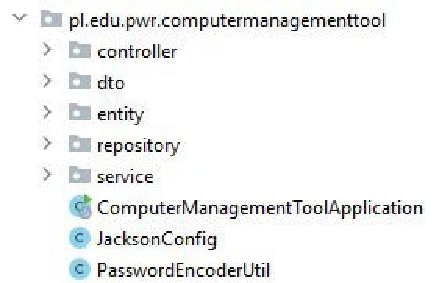
\includegraphics[width=0.33\textwidth]{rys05/backend/ogolne.pdf} & 
	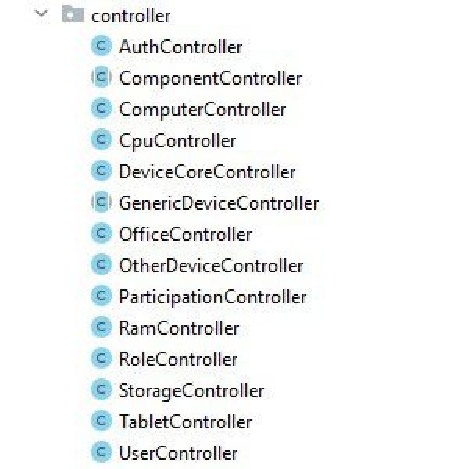
\includegraphics[width=0.33\textwidth]{rys05/backend/controller.pdf} &
	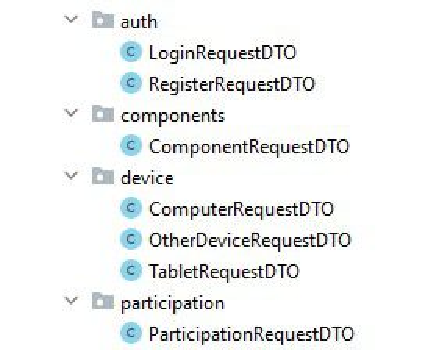
\includegraphics[width=0.33\textwidth]{rys05/backend/dto.pdf} \\

	d) & e) & f) \\
	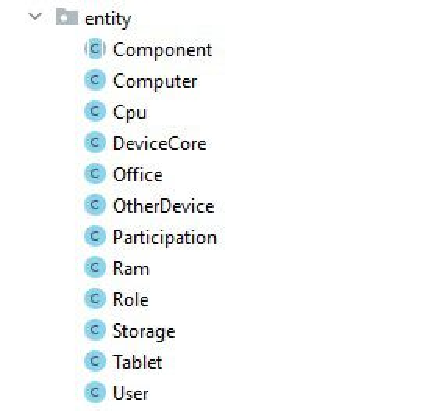
\includegraphics[width=0.33\textwidth]{rys05/backend/entity.pdf} &
	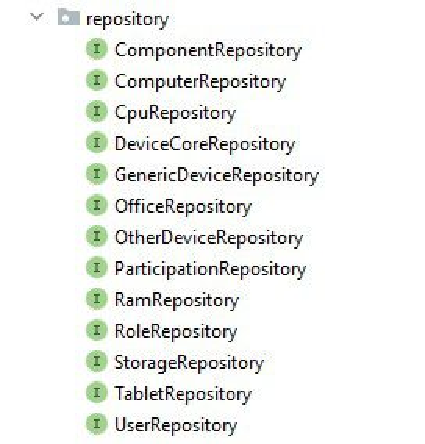
\includegraphics[width=0.33\textwidth]{rys05/backend/repository.pdf} &
	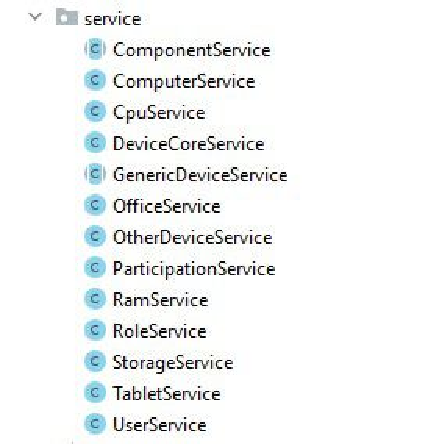
\includegraphics[width=0.33\textwidth]{rys05/backend/service.pdf}
	\end{tabular}
  \caption{Struktura projektu a) ogólna struktura, b) kontrolery, c) data transfer object, d) encje, e) repozytoria, f) serwisy}
  \label{backend_struktura:label}
\end{figure}

\newpage
\subsection{Fragmenty implementacji}
\subsubsection {Fragment kodu klas encji wykorzystującej schemat dziedziczenia}

\begin{lstlisting}[language=Java, style=JavaStyle, caption={Klasa nadrzędna reprezentująca rdzeń sprzętu: DeviceCore}, label={entity_deviceCore}]
@Entity
@Table(name = "device_core")
@Inheritance(strategy = InheritanceType.TABLE_PER_CLASS)
public class DeviceCore {
    @Id
    @GeneratedValue(strategy = GenerationType.TABLE)
    @Column(name = "id", nullable = false)
    private Integer id;

    @Column(name = "device_type", length = 50)
    private String deviceType;

    @Column(name = "device_name", length = 50)
    private String deviceName;
		
		// Pozostała część klasy

\end{lstlisting}
W linii 3 listingu klasy \texttt{DeviceCore} \ref{entity_deviceCore} określono schemat dziedziczenia TABLE\_PER\_CLASS. O sposobie dziedziczenia napisano w podrozdziale \ref{dzedziczenie_hibernate:label}. Linia 3 określa strategie generowania klucza. Hibernate tworzy wtedy specjalną tabelę w bazie danych która odpowiedzialna jest za przechowywanie unikalnych kluczy głownych dla encji sprzętu w aplikacji. W listingu kodu \ref{entity_computer} nie trzeba wtedy definować klucza.

\begin{lstlisting}[language=Java, style=JavaStyle,  caption={Klasa potomna: Computer, reprezentująca komputer}, label={entity_computer}]
@Entity
@Table(name = "computer")
public class Computer extends DeviceCore{

    public static final String DEVICE_TYPE = "COMPUTER";
    @Column(name = "serial_number", length = 50)
    private String serialNumber;

    @Column(name = "operating_system", length = 50)
    private String operatingSystem;

    @Column(name = "battery_life", length = 50)
    private String batteryLife;
		
		// Pozostała część klasy
\end{lstlisting}
W linii 3 określone zostało dziedziczenie po klasie nadrzędnej reprezentującej rdzeń sprzętu. Pola które należy określić w tej klasie są unikalnymi polami tabeli \texttt{computer}. W linii 4 istnieje statyczna zmienna \texttt{DEVICE\_TYPE} która pomaga określić jakiego rodzaju dany sprzęt. Wykorzystywane jest to w aplikacji klienckiej.


\subsubsection{Przykład kodu repozytorium dla urządzeń dziedziczącym po rdzeniu sprzętu}
Repozytorium sprzętu komputerowego zostało napisane z użyciem wyrażeń generycznych. Wykorzystanie ich przyczynia się do uproszczenia kodu oraz łatwiejszej jego rozbudowy.

\begin{lstlisting}[language=Java, style=JavaStyle,  caption={Generyczne repozytorium sprzętu komputerowego:  GenericDeviceRepository}, label={repo_genericDevice}]
@NoRepositoryBean
public interface GenericDeviceRepository<T extends DeviceCore> extends JpaRepository<T, Integer> {
    
    List<T> findAllByReadyToLotteryIsTrue();
    List<T> findAllByOfficeId(int officeId);
}
\end{lstlisting}

W lini 1 adnotacja \texttt{@NoRepositoryBean} jest używana do oznaczenia interfejsów które nie mają mieć swojej instancji. Oznacza to, że nie jest on przeznaczony do utworzenia instancji repozytorium w trakcie uruchomiania aplikacji. W linii 4 i 5 poprzez zdefiniowanie metody możliwe jest wykonanie konkretnego zapytania SQL do bazy danych. Z racji, że klasy sprzętu komputerowego mają zbliżone funkcjonalności nie trzeba dostarczać tych samych interfejsów we wszystkich repozytoriach tylko zastosować schemat dziedziczenia.

\subsubsection{Fragmenty implementacji klasy kontrolerów sprzętu}

\begin{lstlisting}[language=Java, style=JavaStyle,  caption={Klasa nadrzędna kontrolera sprzętu: GenericDeviceController}, label={controller_genericDevice}]
public abstract class GenericDeviceController<T extends DeviceCore> {

    protected final GenericDeviceService<T> genericDeviceService;
    protected final GenericDeviceRepository<T> genericRepository;

    protected GenericDeviceController(GenericDeviceService<T> genericDeviceService, GenericDeviceRepository<T> genericRepository) {
        this.genericDeviceService = genericDeviceService;
        this.genericRepository = genericRepository;
    }

    @GetMapping("/{id}")
    @CrossOrigin(origins = "*")
    T getOneBasicDevice(@PathVariable int id){
        return genericDeviceService.getDeviceById(id);
    }

    @GetMapping("/all")
    @CrossOrigin(origins = "*")
    List<T> getAllBasicDevices(){
        return genericDeviceService.getAllDevices();
    }

    @GetMapping("/all-ready-to-lottery")
    @CrossOrigin(origins = "*")
    List<T> getAllReadyToLotteryDevice(){
        return genericDeviceService.getAllReadyToLotteryDevices();
    }
		
		// Pozostała część klasy
		
		@PutMapping("/set-ready-to-lottery/{id}")
    @CrossOrigin(origins = "*")
    public ResponseEntity<T> setReadyToLottery(@PathVariable int id){
        try{
            T updatedBasicDevice = genericDeviceService.setReadyToLottery(id);
            return new ResponseEntity<>(updatedBasicDevice, HttpStatus.OK);
        } catch (RuntimeException e){
            return new ResponseEntity<>(HttpStatus.NOT_FOUND);
        }
    }
		
		// Pozostała część klasy
		
\end{lstlisting}

Kontrolery pełnią istotną funkcje w systemie. Umożliwiają one definiowanie zapytań REST które będą wysyłane do serwera. Wykorzystując abstrakcje oraz wyrażenia generyczne możliwe jest wykonanie niektórych zapytań bez konieczności ich implementacji w klasach potomnych.


\begin{lstlisting}[language=Java, style=JavaStyle,  caption={Klasa potomna reprezentująca ogólną postać sprzętu}, label={controller_device}]
@RestController
@RequestMapping("/devices")
public class DeviceCoreController extends GenericDeviceController<DeviceCore>{

    protected DeviceCoreController(DeviceCoreService deviceCoreService, GenericDeviceRepository<DeviceCore> genericRepository) {
        super(deviceCoreService, genericRepository);
    }
}
\end{lstlisting}

Powyższa klasa w listingu kodu \ref{controller_device} nie posiada własnych metod. Umożliwia jednak wykonywanie ogólnych operacji dotyczących sprzętu. Możliwe jest między innymi pobranie informacji dotyczące sprzętu bez względu na jego typ co idealnie obrazuje test \ref{getByIdTest:label}


\subsubsection{Fragmenty implementacji klas serwisów sprzętu}


\begin{lstlisting}[language=Java, style=JavaStyle,  caption={Klasa nadrzędna serwisu sprzętu GenericDeviceService}, label={service_tablet}]

public abstract class GenericDeviceService<T extends DeviceCore> {

    protected final GenericDeviceRepository<T> genericDeviceRepository;
    protected final OfficeRepository officeRepository;

    public GenericDeviceService(GenericDeviceRepository<T> genericRepository, OfficeRepository officeRepository) {
        this.genericDeviceRepository = genericRepository;
        this.officeRepository = officeRepository;
    }

    public T getDeviceById(int id) {
        Optional<T> basicDeviceOptional = genericDeviceRepository.findById(id);
        return basicDeviceOptional.orElseThrow(()-> new RuntimeException("Device not found with id: " + id));
    }

    public List<T> getAllDevices() {
        return genericDeviceRepository.findAll();
    }
		// Pozostała część klasy

protected DeviceCore addDevice(Class<? extends DeviceCore> deviceClass, String deviceName, Double price, String description, Integer age, Boolean readyToSell, Integer officeId) {

        if(officeId == null){
            throw new RuntimeException("Office required");
        }
        Optional<Office> officeOptional = officeRepository.findById(officeId);
        Office office = officeOptional.orElseThrow(() -> new RuntimeException("Office not found with id: " + officeId));

        DeviceCore deviceCore;
        try {
            deviceCore = deviceClass.getDeclaredConstructor().newInstance();
        } catch (InstantiationException | IllegalAccessException | NoSuchMethodException | InvocationTargetException e) {
            throw new RuntimeException("Error creating device", e);
        }

        deviceCore.setDeviceName(deviceName);
        deviceCore.setPrice(price);
        deviceCore.setDescription(description);
        deviceCore.setAge(age);
        deviceCore.setReadyToSell(readyToSell);
        deviceCore.setOffice(office);

        return deviceCore;
    }
		
		// Pozostała część klasy

\end{lstlisting}
Serwisy są odpowiedzialne za warstwę logiki biznesowej systemu. W linii 12 widnieje metoda która pozwala na pobranie sprzętu. W linii 17 natomiast jest możliwe pobranie wszystkich sprzętów. Odbywa się to przy pomocy sparametryzowanych typów danych \texttt{T}. Metoda zdefiniowana w linii 22 pozwala uprościć dodawanie sprzętu, implementując część logiki ustawiając parametry charakterystyczne dla rdzenia sprzętu. Jednak aby utworzyć odpowiedni typ niezbędne jest określenie jakiego typu będzie dodawane urządzenie, Dlatego w linii 22 metoda jako parametr przyjmuje \texttt{Class<? extends DeviceCore>} który oznacza typ aplikacji. Tak zdefiniowana metoda może zostać użyta do dodania sprzętu w klasach potomnych co pokazano w listingu \ref{service_tablet}

\begin{lstlisting}[language=Java, style=JavaStyle,  caption={Klasa potomna serwisu tabletu: TabletService }, label={service_tablet}]

@Service
public class TabletService extends GenericDeviceService<Tablet>{

    public TabletService(TabletRepository tabletRepository, OfficeRepository officeRepository){
        super(tabletRepository, officeRepository);
    }

    public Tablet addTablet(String deviceName, Double price, String description,
                            Integer age, String officeAddress,
                            String screenSize, String operatingSystem, String batteryLife){

        Tablet tablet = (Tablet) addDevice(Tablet.class, deviceName, price, description,
                                                                age, officeAddress);

        tablet.setScreenSize(screenSize);
        tablet.setOperatingSystem(operatingSystem);
        tablet.setDeviceType(Tablet.DEVICE_TYPE);
        tablet.setBatteryLife(batteryLife);

        return genericDeviceRepository.save(tablet);
    }
		// Pozostała część klasy
\end{lstlisting}

Serwis klasy \texttt{TabletService} dziedziczy i parametryzuje metody klasy \texttt{GenericDeviceService}. Wykorzystuje on w linii 13 metodę klasy nadrzędnej co uprasza implementacje metody dodającej sprzęt(linia 9)



\section {Aplikacja kliencka}
Aplikacja kliencka jest aplikacją internetową dostarczającą przyjazny interfejs użytkownika. W aplikacji klienckiej napisanej w języku JavaScript z wykorzystaniem biblioteki React (tabela \ref{tab:zestawienie_narzędzi}) istnieją zdefiniowane zapytania REST do aplikacji serwerowej. Wykorzystując te zapytania na widoku widocznym dla użytkownika zostają podjęte specjalne akcje które ten widok aktualizują. Formularze pokazywane są w takiej formie, że po kliknięciu odpowiedniego przycisku ukazuje się formularz na danym widoku. Zestawienie widoków, ścieżek i roli pokazano w tabeli \ref{tab:zestawienie_widokow}

\subsection{Struktura projektu}
Ogólna struktura projektu została stworzona przez wywołanie komendy tworzącej aplikacje Reacta: \texttt{npx create-react-app frontend}. Następnie utworzono folder \texttt{components} który w sobie zawiera foldery przechowujące pliki JavaScript na podstawie pełnionych funkcji w projekcie. Foldery i odpowiadające im funkcje: 
\begin {itemize}
\item \texttt{\textbf{auth}} przechowuje pliki odpowiedzialne za obsługę i stylizacje widoków logowania i rejestracji
	\begin{itemize}
	\item \texttt{Login.js} -- skrypt odpowiedzialny za widok i funkcjonalność logowania
	\item \texttt{Register.js} -- skrypt odpowiedzialny za widok i funkcjonalność rejestracji
	\item \texttt{Login.css} -- arkusz styli odpowiedzialny za stylizacje widoków logowania i rejestracji
	\end{itemize}
\item \texttt{\textbf{bar}} przechowuje skrypty odpowiedzialne za paski nawigacyjne poszczególnych widoków.
	\begin{itemize}
	\item \texttt{AdminHomeBar.js} -- skrypt odpowiedzialny za pasek nawigacyjny na widoku domowym administratora: \texttt{Home.js}
	\item \texttt{ComputerComponentsBar.js} -- skrypt odpowiedzialny za pasek nawigacyjny dla widoku komponentów: \texttt{ComputerComponents.js}
	\item \texttt{ManageUserBar.js} -- skrypt odpowiedzialny za pasek nawigacyjny widoku zarządzania użytkownikami: \texttt{Users.js}
	\item \texttt{UserHomeBar.js} -- skrypt odpowiedzialny za pasek nawigacyjny na widoku domowym pracownika: \texttt{Home.js}
	\item \texttt{UserLotteryHistory} -- skrypt odpowiedzialny za pasek nawigacyjnym na widoku historii loterii użytkownika: \texttt{UserLotteryHistory.js}
	\item \texttt{UsersInLottery.js} -- skrypt odpowiedzialny za pasek nawigacyjny na widoku użytkowników biorących udział w loterii: \texttt{UsersInLottery.js}
	\end{itemize}
\item \texttt{\textbf{computer\_components}} przechowuje skrypty formularzy komponentów komputera które mogą dodawać lub modyfikować te komponenty
	\begin{itemize}
	\item \texttt{CpuForm.js} -- formularz procesora
	\item \texttt{RamForm.js} -- formularz pamięci RAM
	\item \texttt{StorageForm.js} -- formularz pamięcu dyskowej
	\end{itemize}
\item \texttt{\textbf{device\_form}} przechowuje skrypty oraz arkusz styli odpowiedzialne za logikę formularzy dodawania, modyfikacji urządzeń
	\begin{itemize}
	\item \texttt{AddNewFormPopup.js} -- formularz umożliwiający wybór formularza który dodaje komputer, tablet, lub inne urządzenie
	\item \texttt{ComputerForm.js} -- formularz komputera
	\item \texttt{DeviceForm.css} -- arkusz styli odpowiedzialny za stylizacje formularzy
	\item \texttt{FormPopup.js} -- skrypt odpowiedzialny za logikę i wybór rodzaju formularza(dodawanie, modyfikacja, informacje) urządzenia.
	\item \texttt{OtherDeviceForm} -- formularz innego urządzenia
	\item \texttt{TabletForm.js} -- formularz tabletu
	\end{itemize}
\item \texttt{\textbf{view}} przechowuje w sobie skrypty oraz arkusz styli odpowiedzialne za widoki aplikacji
	\begin{itemize}
	\item \texttt{ComputerComponets.js} -- widok dostępny tylko dla administratora. Zawiera w sobie informacje o komponentach komputera w postaci tabeli
	\item \texttt{Home.css} -- arkusz styli odpowiedzialny za stylizacje widoków
	\item \texttt{Home.js} -- widok strony domowej, ma w sobie dwa warianty: Administratora i Pracownika
	\item \texttt{UserLotteryHistory.js} -- widok historii loterii użytkownika o zadanym ID. Dostępny dla pracownika i administratora.
	\item \texttt{Users.js} -- widok pracowników zarejestrowanych w systemie. Dostępny tylko dla administratora
	\item \texttt{UsersInLottery} -- widok pracowników biorących udział w loterii danego sprzętu. Dostępny tylko dal administratora.
	\end{itemize}
\end{itemize}

Równolegle do folderu \texttt{components} w folderze \texttt{src} istnieją jeszcze dwa skrypty które są niezbędne do funkcjonowania aplikacji.
\begin{itemize}
	\item \texttt{App.js} zawiera w sobie scieżki url pod którymi dostępne są poszczególne widoki
	\item \texttt{index.js} -- funkcja główna programu
\end{itemize}

Strukturę projektu pokazano na rysunku \ref{frontend_struktura:label}


\begin{table}[htb] \small
	\centering
\caption{Zestawienie ścieżek url dostępnych w aplikacji klienckiej}
\label{tab:zestawienie_widokow}
\begin{tabularx}{\linewidth}{|X|X|X|X|}
    \hline
    Ścieżka & Widok & Skrypt & Rola\\
    \hline \hline
    /auth/login & Logowanie &  Login.js & Przed nadaniem roli\\
    \hline
    /auth/register & Rejestracja & Register.js & Przed nadaniem roli\\
    \hline
    /home & Strona domowa z tabelą sprzętów & Home.js & Administrator lub Pracownik\\
    \hline
    /users & Tabela pracowników & Users.js & Administrator\\
    \hline
		/components & Tabela komponentów komputera& ComputerComponents.js & Administrator\\
    \hline
		/users-in-lottery & Tabela użytkowników biorących udział w loterii& UsersInLottery.js & Administrator lub Pracownik\\
    \hline
		/users-lottery-history & Tabela zawierająca historię loteri & UsersLotteryHistory.js & Administatro lub Pracownik\\

    \hline
\end{tabularx}
\end{table}


\begin{figure}[htb]
  \centering
	\begin{tabular}{@{}lll@{}}
	a) & b) & c) \\
  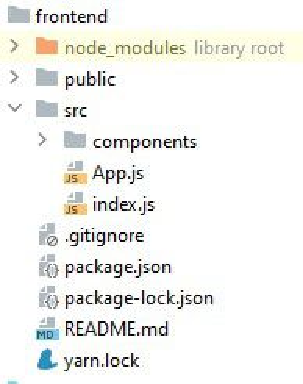
\includegraphics[width=0.3\textwidth]{rys05/frontend/frontend.pdf} & 
	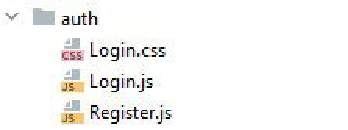
\includegraphics[width=0.3\textwidth]{rys05/frontend/auth.pdf} &
	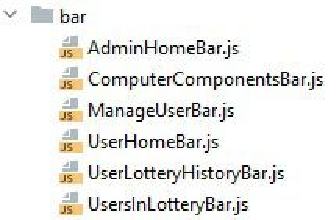
\includegraphics[width=0.3\textwidth]{rys05/frontend/bar.pdf} \\

	d) & e) & f) \\
	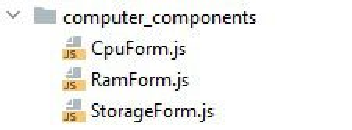
\includegraphics[width=0.3\textwidth]{rys05/frontend/components.pdf} &
	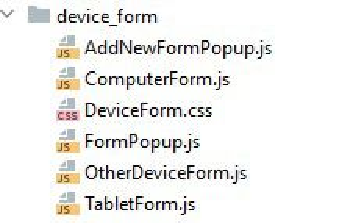
\includegraphics[width=0.3\textwidth]{rys05/frontend/deviceform.pdf} &
	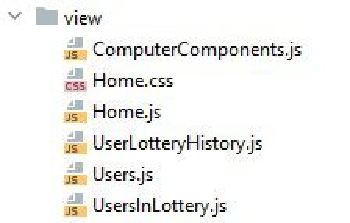
\includegraphics[width=0.3\textwidth]{rys05/frontend/view.pdf}
	\end{tabular}
  \caption{Struktura projektu a) ogólna struktura, b) Logowanie i rejestracja, c) pasek nawigacyjny, d) formularze komponentów, e) formularze sprzętów, f) widoki stron}
  \label{frontend_struktura:label}
\end{figure}



\subsection{Fragmenty implementacji}
	\subsubsection{Ścieżki url dla widoków aplikacji}
	

\begin{lstlisting}[language=JavaScript, style=JavaScriptStyle,  caption={Zdefiniowane ścieżki url widoków systemu }, label={app_frontend:label}]
	
	const App = () => {
    return (
        <Router>
            <Routes>
                <Route path="/auth/login" element={<Login />} />
                <Route path="/auth/register" element={<Register />} />
                <Route path="/home" element={<Home />} />
                <Route path="/" element={<Navigate to="/auth/login" />} />
                <Route path="/auth/*" element={<Navigate to="/auth/login" />} />
                <Route path="/users" element={<Users/>}/>
                <Route path="/components" element={<ComputerComponents/>}/>
                <Route path="/users-in-lottery" element={<UsersInLottery/>}/>
                <Route path="/user-lottery-history" element={<UserLotteryHistory/>}/>
            </Routes>
        </Router>
    );
};
	
\end{lstlisting}
Powyższy listing kodu \ref{app_frontend:label} definiuje ścieżki url pod którymi dostępne są poszczególne widoki~\ref{tab:zestawienie_widokow}


\subsubsection{Sparametryzowany formularz urządzenia}

\begin{lstlisting}[language=JavaScript, style=JavaScriptStyle,  caption={Obsługa formularzy}, label={render_data:label}]

function FormPopup(props){
    
 const {setTrigger, formType, deviceType, deviceId} = props;
    
  return (props.trigger) ? (
    <div className="popup">
      <div>
         {deviceType === 'COMPUTER' && <ComputerForm setTrigger={props.setTrigger} formType={formType} deviceId={deviceId}/>}
         {deviceType === 'TABLET' && <TabletForm setTrigger={props.setTrigger} formType={formType} deviceId={deviceId}/>}
         {deviceType === 'OTHER' && <OtherDeviceForm setTrigger={props.setTrigger}  formType={formType} deviceId={deviceId} />}
         {props.children}
      </div>
    </div>
 ) : "";
}

export default FormPopup
										
\end{lstlisting}

Powyższy listing kodu \ref{render_data:label} dla skryptu \texttt{FormPopup.js}  służy do dodawania różnych rodzajów formularza sprzętów z różnymi wariantami. Przyjmuje 4 argumenty. Przekazywanie tych parametrów odbywa się w linii 4 z wykorzystaniem "`\texttt{props}"'. Zmienna \texttt{deviceType} odpowiada dla jakiego urządzenia dotyczy formularz. Może on dotyczyć komputera, tabletu lub innego urządzenia co pokazano w liniach 9-11. Zmienna \texttt{setTrigger} jest odpowiedzialna za to czy formularz jest aktualnie wyświetlany nad widokiem. Zmienna \texttt{formType} dotyczy wariant formularza. Istnieją 3 warianty jednego formularza i dotyczą one kolejno: dodawania nowego sprzętu, modyfikacji sprzętu oraz wyświetlania informacji o sprzęcie. Warianty formularza pokazano rysunku \ref{forms:label}. Tak stworzona funkcja umożliwia zarządzanie formularzami które zostały zdefiniowane w plikach \texttt{ComputerForm.js}, \texttt{TabletForm.js} oraz \texttt{OtherDeviceForm.js}.

\begin{lstlisting}[language=JavaScript, style=JavaScriptStyle,  caption={Przykładowe zapytanie do serwera dla formularza komputera}, label={addComputer:label}]

const handleAddComputer = async (e) =>{

        try{
            const compData ={
                "deviceName" : formData.deviceName,
                "price" : formData.price,
                "description" : formData.description,
                "age" : formData.age,
                "officeAddress" : formData.office,
                "serialNumber" : formData.serialNumber,
                "model" : formData.model,
                "operatingSystem" : formData.model,
                "batteryLife" : formData.batteryLife,
                "cpuName" : formData.cpu,
                "storageName" : formData.storage,
                "ramName" : formData.ram
            };

            const response = await axios.post('http://localhost:8080/computers/add', compData, {

            });

        }catch (error){
            console.error('Bład dodawania komputera', error)
        }

\end{lstlisting}

Powyższy listing kodu \ref{addComputer:label} ukazuje w jaki sposób aplikacje kliencka komunikuje się z serwerem. Po podaniu odpowiednich danych w formularzu i kliknięciu przycisku następuje wysłanie żądania typu POST do serwera które dodaje nowy komputer. 

\subsection{Instrukcja użytkowania}

Zdefiniowano widoki aplikacji i pogrupowano je ze względu na typ które pełnią.
\begin{itemize}
	\item W-1 -- widok logowania i rejestracji, rysunek \ref{authview:label}
	\item W-2 -- widok strony domowej zawierający urządzenia oraz loterię tych urządzeń, rysunek \ref{home:label}
	\item W-3 -- widok formularzy urządzeń z wariantami dotyczących funkcjonalności które pełnią, rysunek \ref{forms:label}
	\item W-4 -- widok użytkowników i uczestników, rysunek \ref{manageUsers:label}
	\item W-5 -- widok historii loterii użytkownika, rysunek \ref{lotteryHistory:label}
	\item W-6 -- widok komponentów komputera, rysunek \ref{components:label}
	\item W-7 -- widok formularzy komponentów komputera, rysunek \ref{compforms:label}
\end{itemize} 





\begin{figure}[htb]
  \centering
	\begin{tabular}{@{}ll@{}}
	a) & b) \\
  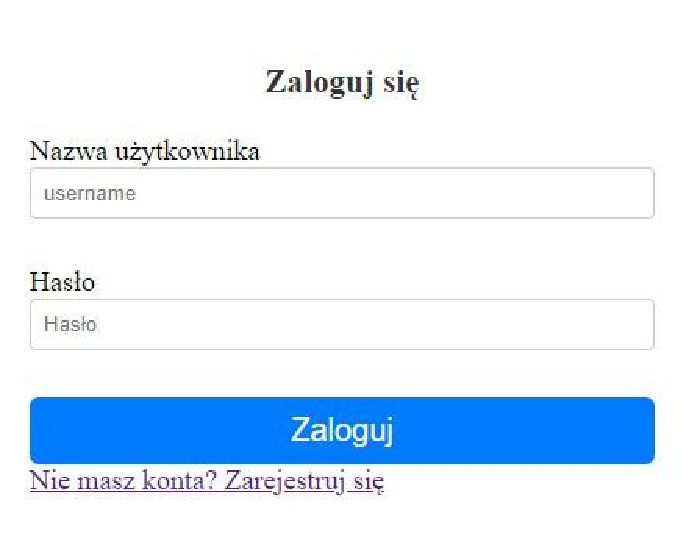
\includegraphics[width=0.35\textwidth]{rys05/view/login.pdf} & 
	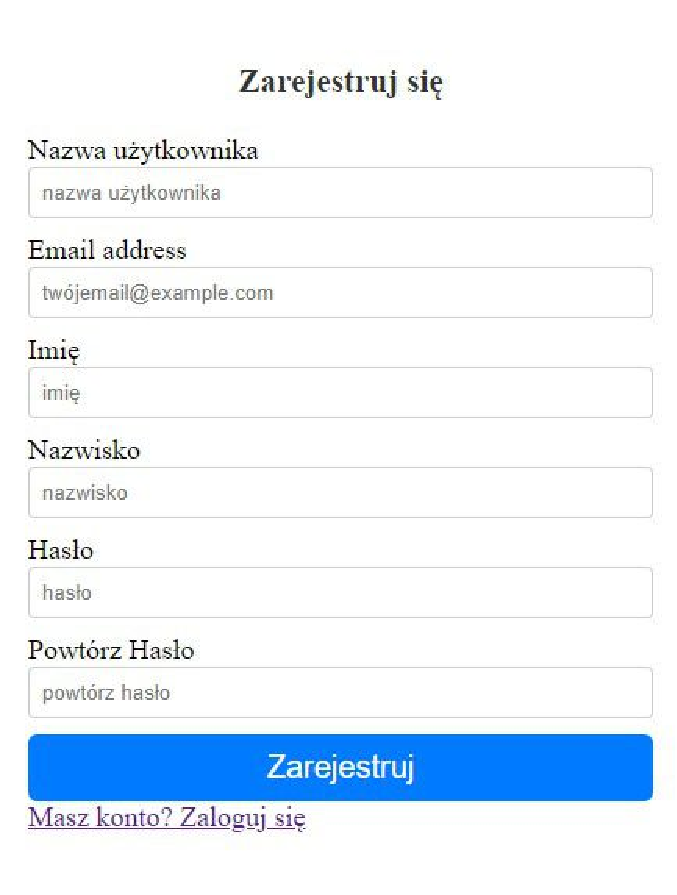
\includegraphics[width=0.35\textwidth]{rys05/view/register.pdf}
	\end{tabular}
  \caption{Widok W-1, Logowanie i Rejestracja a) logowanie, b) rejestracja}
  \label{authview:label}
\end{figure}


Widok W-1 formularzy logowania i rejestracji pokazany na rysunku \ref{authview:label} jest początkowym widokiem aplikacji. Każdy użytkownik musi się zalogować podając poprawne dane logowania na W-1a. W przypadku braku konta możliwa jest rejestracja klikając na odnośnik "`Nie masz konta? Zarejestruj się"' Po kliknięciu odnośnika następuje przekierowanie na W-1b. Po pomyślnym zarejestrowaniu następuje przekierowanie do W-1a. Możliwe jest tez kliknięcie odnośnika "`Masz już konto? Zaloguj się"' aby przejśc do formularza logowania W-1a.



\begin{figure}[htb]
  \centering
	\begin{tabular}{@{}lll@{}}
	a)\\
  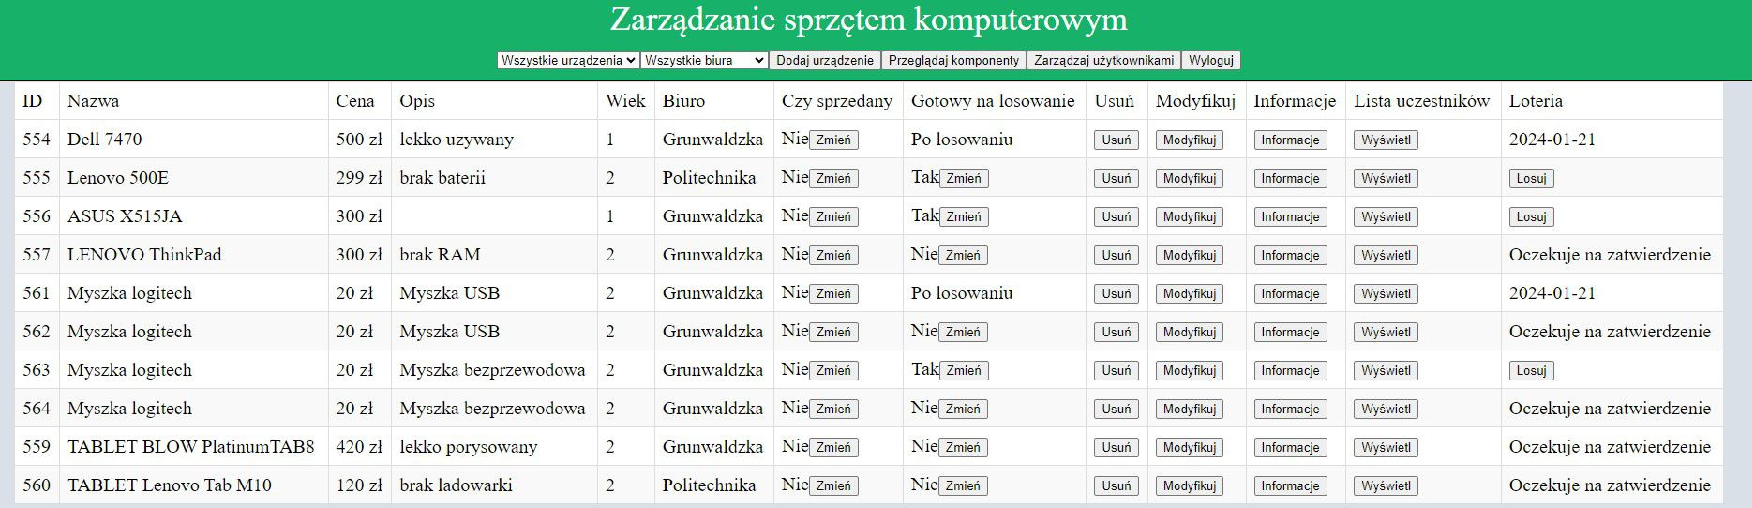
\includegraphics[width=\textwidth]{rys05/view/alldevices.pdf} \\
	
	b)\\
	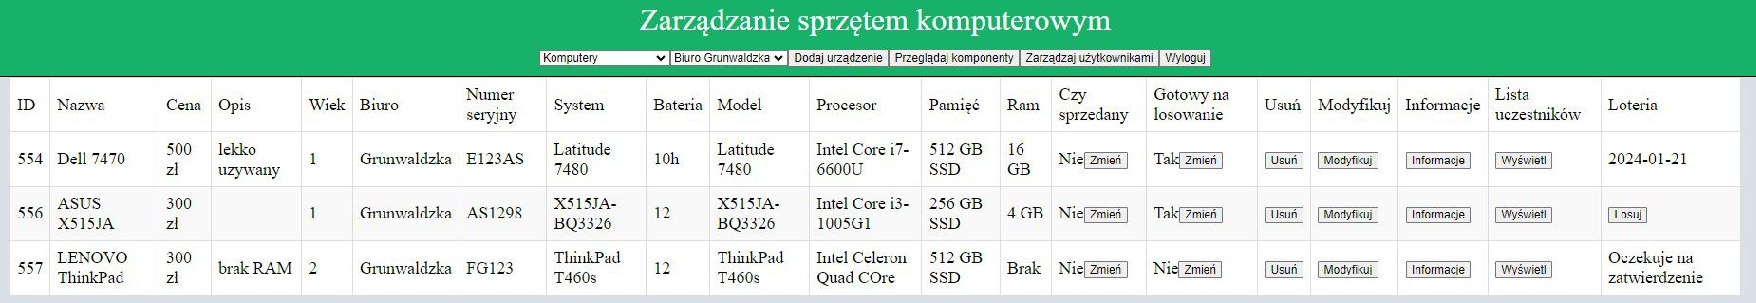
\includegraphics[width=\textwidth]{rys05/view/compGrun.pdf} \\
	c) \\
	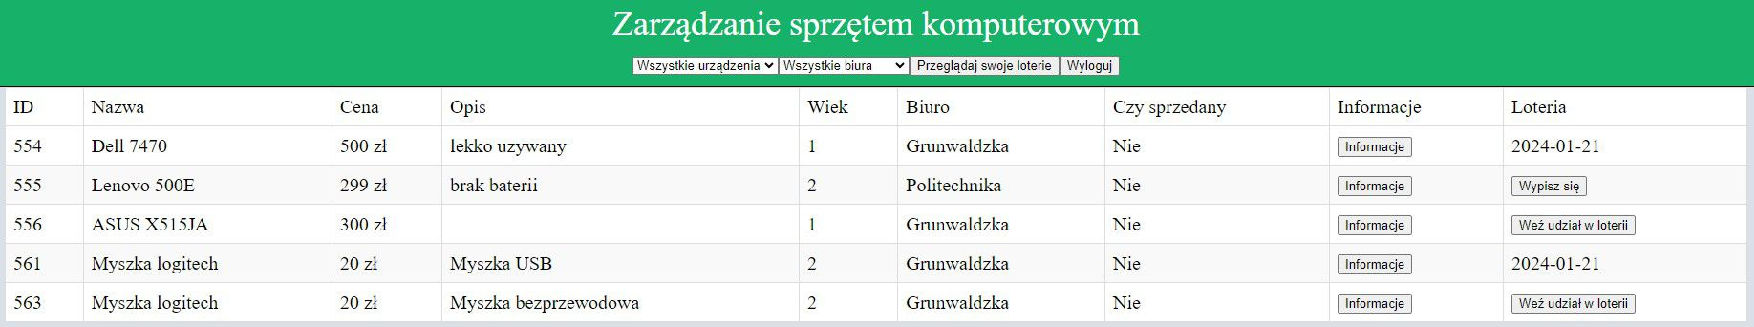
\includegraphics[width=\textwidth]{rys05/view/pracownikHome.pdf}
	\end{tabular}
  \caption{Widok W-2, Strona domowa a)Administrator bez filtrowania, b)Administrator z filtrowaniem c) Pracownik bez filtrowania}
  \label{home:label}
\end{figure}


Na rysunkach \ref{home:label} pokazany jest widok W-2 który posiada tabelę urządzeń z loteriami. Na każdym widoku istnieje przycisk wyloguj odpowiedzialny za wylogowywanie i przekierowanie do widoku W-1a \ref{authview:label}.Na widokach stron domowych W-2 możliwe jest filtrowanie urządzeń po typie urządzenia oraz po biurze w którym się znajdują oraz wyświetlanie szczegółowych informacji o urządzeniu. W widoku W-2b pokazane zostały tylko komputery które znajdują się w biurze Grunwaldzka. Wyświetlanie informacji o urządzeniu pokazuje na widoku wariant formularza W-3e dla odpowiadającego typu urządzenia: W-3a, W-3b, W-3c, rysunek \ref{forms:label}. Widok W-1a jest widokiem administratora który posiada wiele funkcjonalności:
\begin{itemize}
	\item Kliknięcie przycisku "`Dodaj urządzenie"' sprawia, że na ekranie wyświetlany jest formularz W-3a. Możliwa jest zmiana typu formularza na W-3b lub W-3c, która się odbywa poprzez wybór typu urządzenia z listy rozwijanej.
	\item Kliknięcie przycisku "`Przeglądaj komponenty"' sprawia, że następuje przekierowanie do widoku komponentów W-6.
	\item Kliknięcie przycisku "`Zarządzaj użytkownikami"' przekierowuje do widoku zarejestrowanych pracowników W-4a, rysunek \ref{manageUsers:label}
	\item Kliknięcie przycisku "`Zmień"' w kolumnie czy sprzedany ustawia status sprzętu na sprzedany lub nie. Jest to informacja czy sprzęt został dostarczony do pracownika.
	\item Kliknięcie przycisku w kolumnie "`Gotowy na losowanie"' możliwe jest tylko wtedy gdy losowanie się nie odbyło. Sprawia ono, że operacja "`Losuj"' w kolumnie loteria jest możliwa. Sprzęty które mają status gotowe do losowania są wyświetlane na widoku pracownika W-2c.
	\item Kliknięcie przycisku "`Usuń"' usuwa z systemu odpowiedni sprzęt.
	\item Kliknięcie przycisku "`Modyfikuj"' wyświetla na widoku wariant formularza W-3d, rysunek \ref{forms:label}. Wariant ten jest dostosowywany na podstawie odpowiadającemu mu rodzajowi sprzętu: W-3a, W-3b, W3-c.
	\item Kliknięcie przycisku "`Wyświetl"' w kolumnie "`Lista uczestników"' przekierowuje do widoku pracowników biorących udział w loterii wybranego sprzętu W-4b \ref{manageUsers:label}
	\item Kliknięcie przycisku "`Losuj"' w kolumnie loteria możliwe jest w przypadku gdy urządzenie jest gotowe do losowania oraz loteria się jeszcze nie odbyła. Następnie po kliknięciu przycisku ustawiana data losowania jest na dzisiejszą oraz losowany jest zwycięzca losowania. W przypadku braku uczestników losowanie nie odbędzie się.
\end{itemize}
Widok W-2c \ref{home:label} jest widokiem pracownika. Nie posiada on tak zaawansowanych funkcjonalności jak administrator. 
\begin{itemize}
	\item Kliknięcie przycisku w kolumnie loteria umożliwia zapisywanie lub wypisywanie z uczestnictwa w losowaniu. Zapis na loterie możliwy jest wtedy kiedy losowanie się jeszcze nie odbyło.
	\item Kliknięcie przycisku "`Przeglądaj swoje loterie"' przekierowuje do widoku W-5, rysunek \ref{lotteryHistory:label}. Widok ten posiada historię loterii dla aktualnie zalogowanego użytkownika.
\end{itemize}



\begin{figure}[htb]
  \centering
	\begin{tabular}{@{}l@{~}l@{~}l@{}}
	a) & b) & c) \\
	\vtop{\vskip-2ex\hbox{\fbox{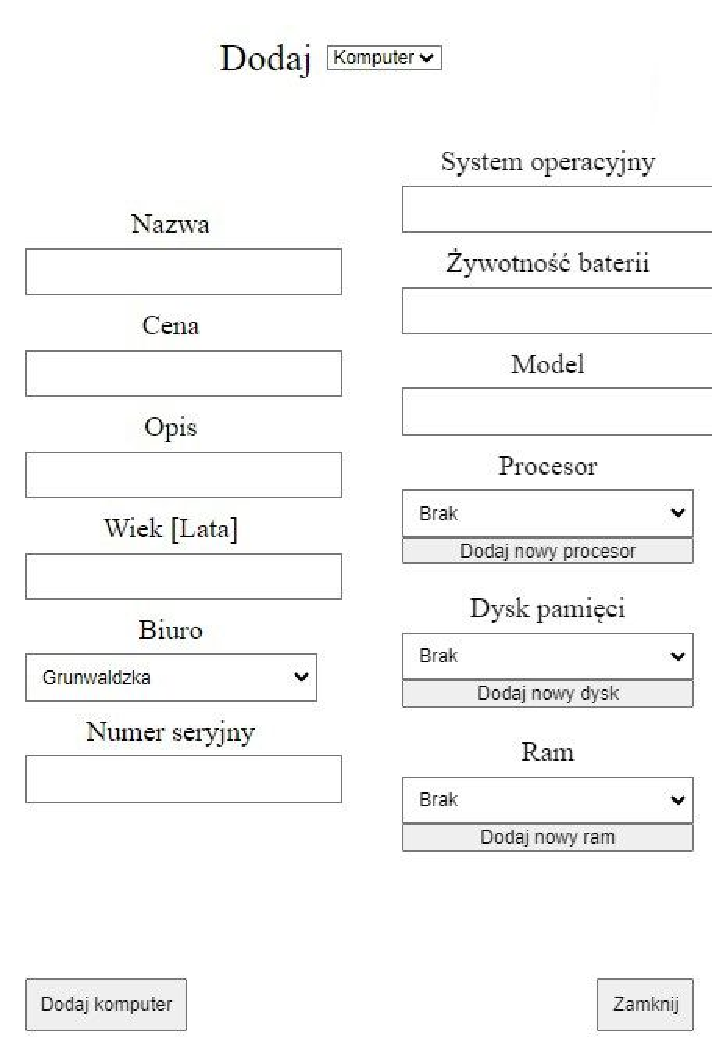
\includegraphics[width=0.3\linewidth]{rys05/view/addComputer.pdf}}}} & 
	\vtop{\vskip-2ex\hbox{\fbox{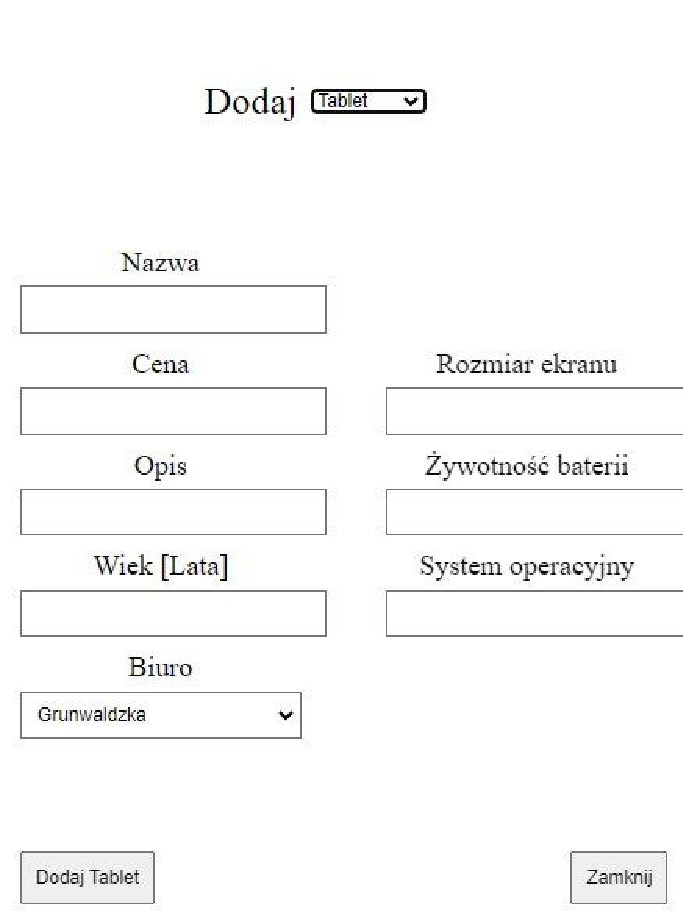
\includegraphics[width=0.3\linewidth]{rys05/view/addTablet.pdf}}}} & 
	\vtop{\vskip-2ex\hbox{\fbox{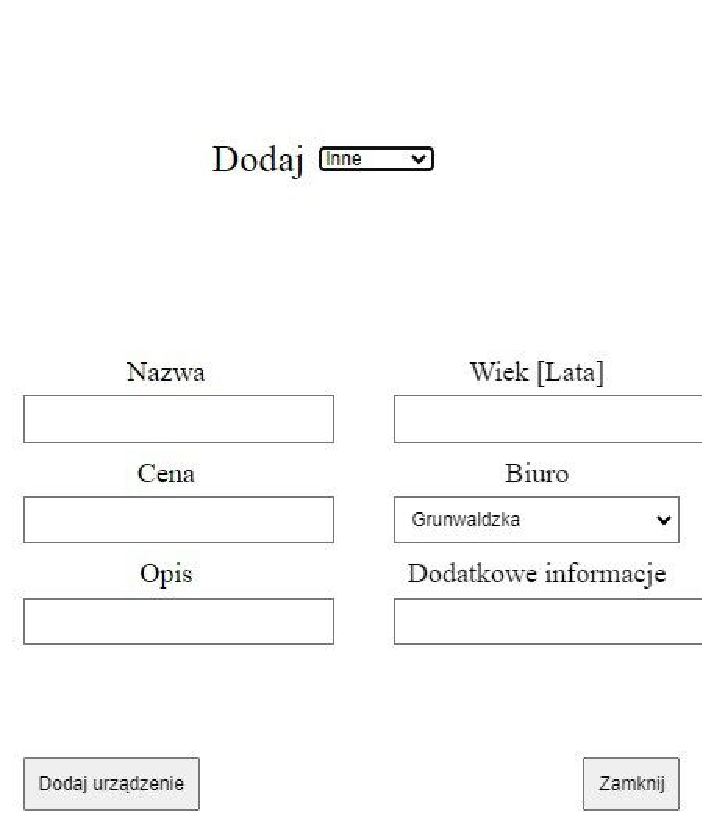
\includegraphics[width=0.3\linewidth]{rys05/view/addInne.pdf}}}} \\
 
	d) & e) \\
	
	\vtop{\vskip-2ex\hbox{\fbox{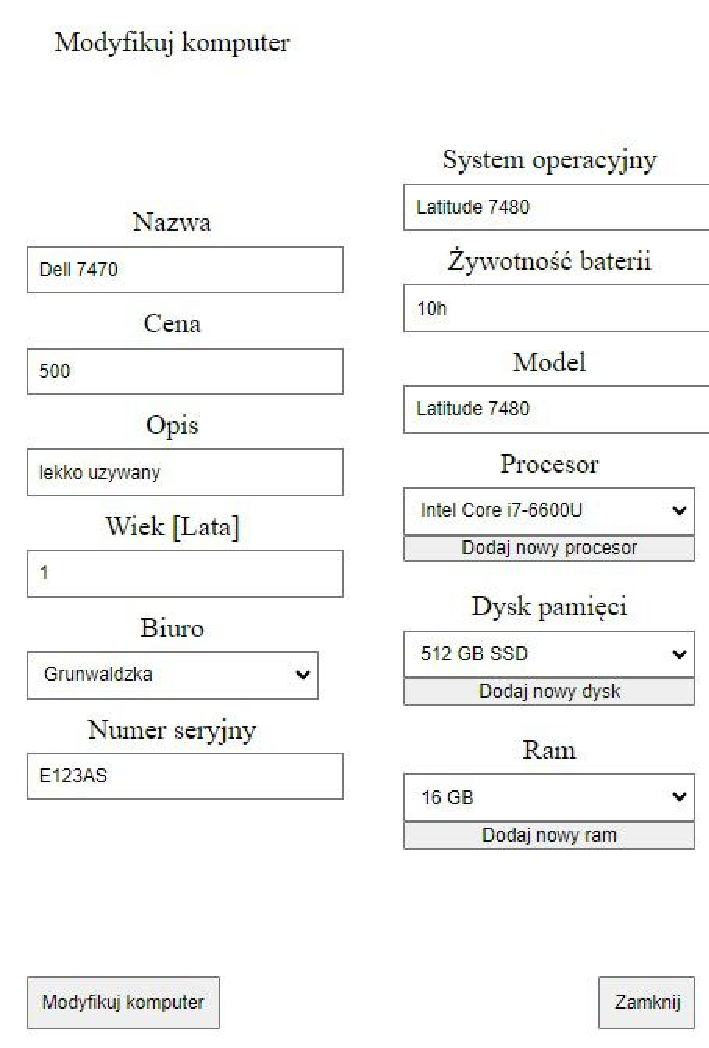
\includegraphics[width=0.3\linewidth]{rys05/view/modifyComp.pdf}}}} & 
	\vtop{\vskip-2ex\hbox{\fbox{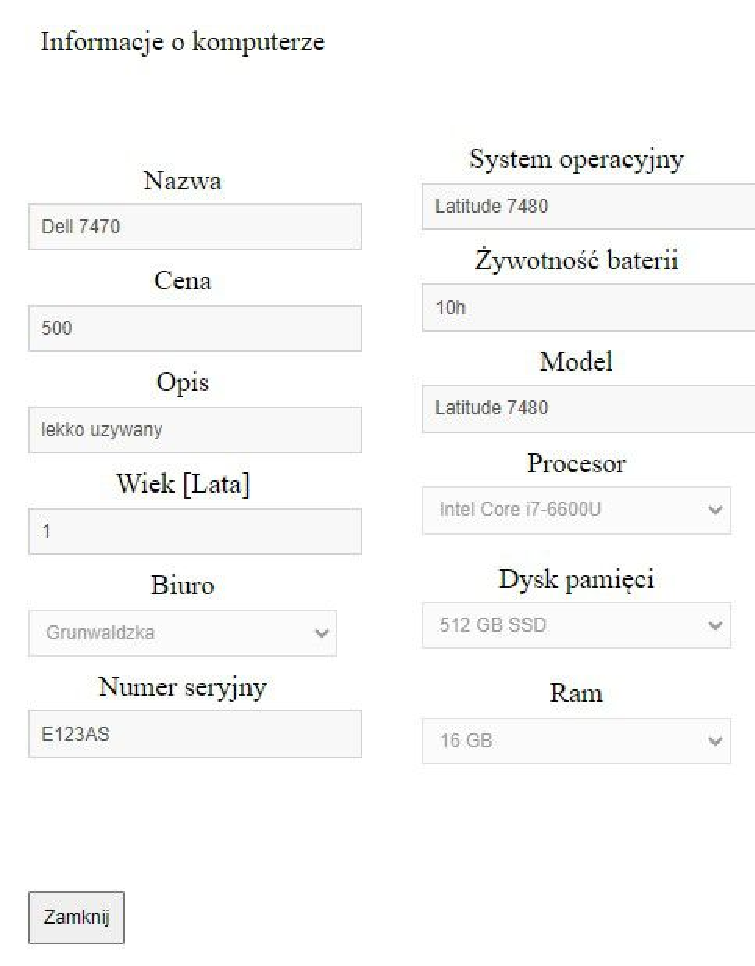
\includegraphics[width=0.3\linewidth]{rys05/view/infoComp.pdf}}}} & 
 
	\end{tabular}
  \caption{Widok W-3, Formularze a) dodawania komputera, b) dodawania tabletu, c) dodawania innego sprzętu, d) wariant modyfikacji, e) wariant informacji}
  \label{forms:label}
\end{figure}


Formularze W-3 ukazane na rysunku \ref{forms:label} wyświetlane są jako wyskakujące okno. Każdy z trzech formularzy W-3a, W-3b, W-3c oprócz wersji podstawowej odpowiadający mu wariant W-3d i W3e. Wariant podstawowy W-3a, W-3b, W-3c odpowiada za dodawanie nowego sprzętu. Możliwa jest zmiana typu sprzętu wybierając opcje z listy rozwijanej. Wariant W-3d służy to modyfikacji urządzenia i po jego pojawieniu się posiada aktualne dane urządzenia. Wariant W-3e odpowiada za wyświetlanie informacji o urządzeniu. Możliwość zmieniania danych na tym formularzu jest zablokowana. Formularz W-3a oraz odpowiadający mu W-3d posiada przyciski "`Dodaj nowy procesor"', "`Dodaj nowy dysk"', "`Dodaj nowy ram"'. W przypadku gdy administrator nie znajdzie z list rozwijanych interesującego go komponentu może kliknąć odpowiedni przycisk. Kliknięcie to powoduje pojawienie się formularza dla odpowiadającego go przycisku W-7a, W-7b, W-7c, rysunek \ref{compforms:label} Po dodaniu komponentu z widoku W-7 możliwe jest teraz z listy rozwijanej wybranie dodanego komponentu. \newline



\begin{figure}[htb]
  \centering
	\begin{tabular}{@{}lll@{}}
	a)\\
  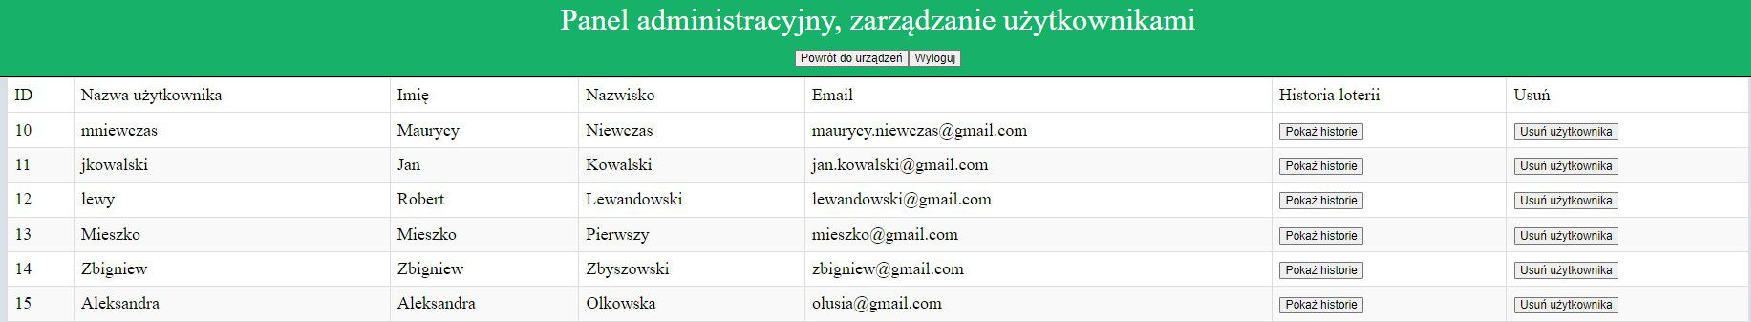
\includegraphics[width=\textwidth]{rys05/view/manageUsers.pdf} \\
	
	b)\\
	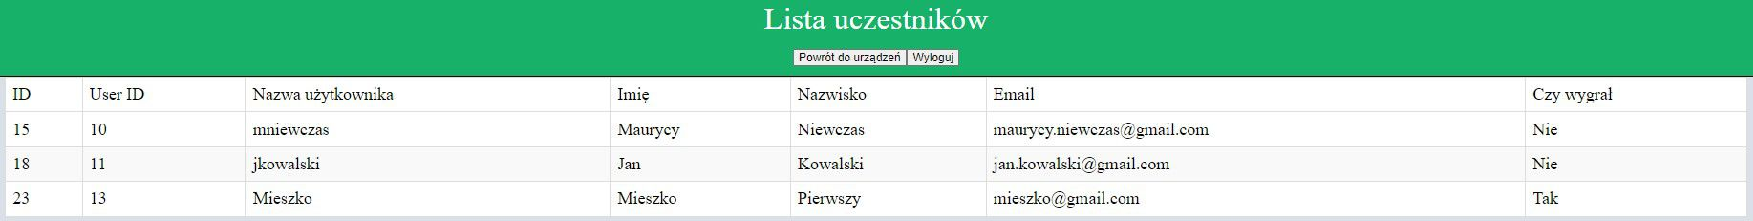
\includegraphics[width=\textwidth]{rys05/view/participation.pdf} \\
	
	\end{tabular}
  \caption{Widok W-4, Informacje o uzytkownikach a)Zarządzanie użytkownikami przez administratora, b)Przeglądanie uczestników losowania}
  \label{manageUsers:label}
\end{figure}


Widok W-4 \ref{manageUsers:label} posiada informacje o użytkownikach. W-4a jest widokiem dostępnym tylko dla administratora
\begin{itemize}
	\item kliknięcie przycisku powrót do urządzeń przekierowuje do strony domowej W-2 \ref{home:label}
	\item kliknięcie przycisku "`Pokaż historię"' w kolumnie Historia loterii przekierowuje do widoku historii loterii  W-5 \ref{lotteryHistory:label} dla odpowiadającego pracownika
	\item kliknicie przycisku "`Usuń użytkownika"' usuwa z systemu użytkownika
\end{itemize}
Widok W-4b też jest widokiem tylko dostępnym dla administratora. Posiada on listę uczestników oraz informacje o wygranej przegranej każdego poszczególnego uczestnika dla wybranej loterii.\newline


\begin{figure}[h]
		\centering
    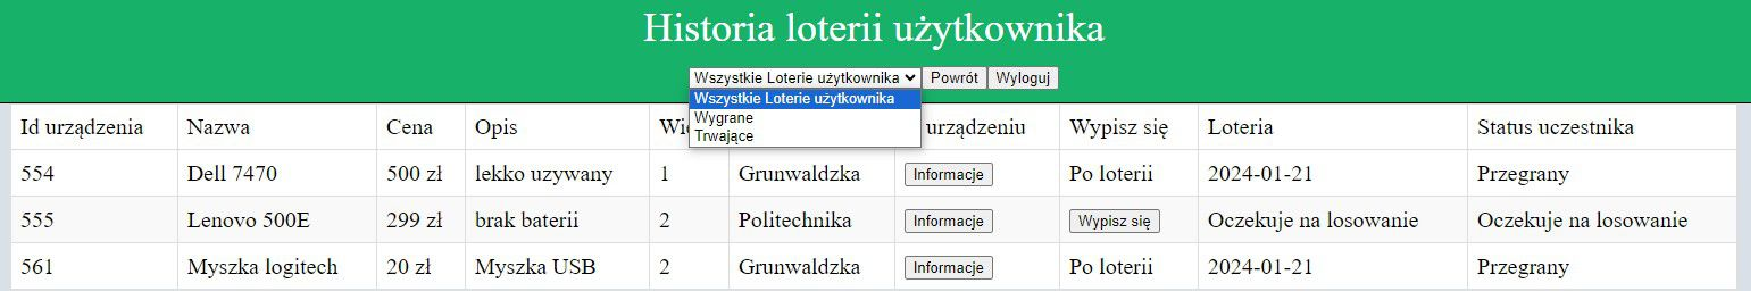
\includegraphics[width=\linewidth]{rys05/view/lotteryHistory.pdf}
    \caption{Widok W-5, Historia loteri pracownika}
    \label{lotteryHistory:label}
\end{figure}


Widok W-5 pozwala wyświetlić historię loterii użytkownika, rysunek \ref{lotteryHistory:label}. Pozwala on na pracownikowi przeglądanie własnej historii. Administrator może skorzystać z tego widoku aby sprawdzić historię loterii wybranego pracownika.
\begin {itemize}
	\item Możliwe jest tutaj filtrowanie loterii na podstawie statusu uczestnika. Są dostępne 3 opcje: "`Wszystkie loterie użytkownika"', "`Wygrana"' i "`Trwająca"'
	\item Kliknięcie przycisku "`Informacje"' wyświetla szczegółowe informacje o sprzęcie, wariant W-3e dla formularzy W-3a, W-3b, W-3c, rysunek \ref{forms:label} 
	\item Kliknięcie przycisku "`Wypisz się"' możliwe jest wtedy kiedy loteria się jeszcze nie odbyła. Po kliknięciu tego przycisku pracownik rezygnuje z uczestnictwa w losowaniu wybranego sprzętu.
\end{itemize} 




\begin{figure}[h]
		\centering
    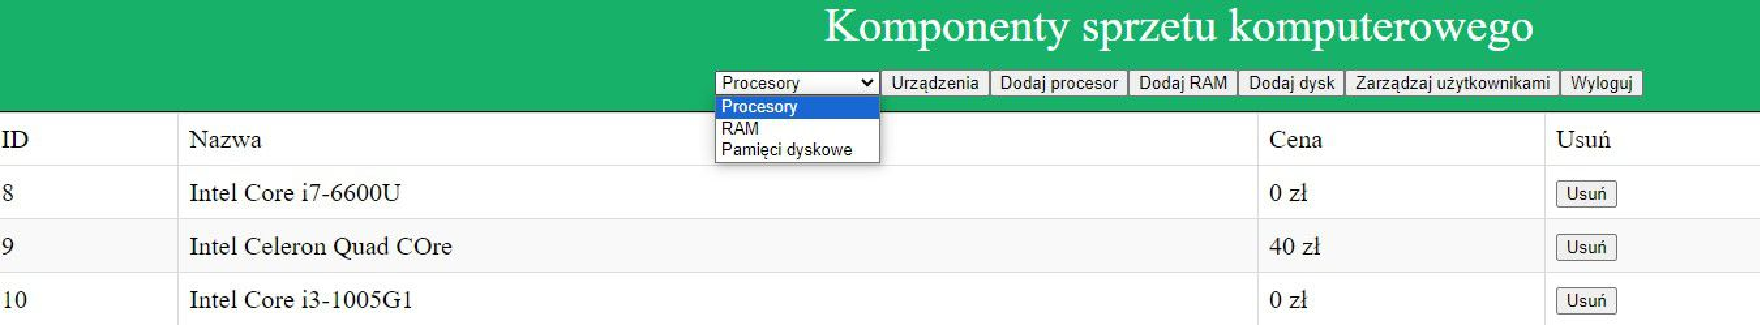
\includegraphics[width=\linewidth]{rys05/view/components.pdf}
    \caption{Widok W-6, Widok komponentów komputera}
    \label{components:label}
\end{figure}

Widok W-6 jest dostępny dla administratora. Pozwala mu na oszacowanie ceny sprzętu patrząc jakie komponenty mają cenę. Możliwe jest wybranie z listy rozwijanej jakiego rodzaju komponenty mają być wyświetlane. Do wyboru są: procesory, pamięci RAM oraz pamięci dyskowe.
\begin{itemize}
	\item Kliknięcie przycisku "`Dodaj procesor"' wyświetli formularz W-7a \ref{compforms:label} odpowiedzialny za dodanie procesora.
	\item Kliknięcie przycisku "`Dodaj RAM"' Wyświetli formularz W-7b \ref{compforms:label} odpowiedzialny za dodanie pamięci RAM.
	\item Kliknięcie przycisku "`Dodaj dysk"' Wyświetli formularz W-7c \ref{compforms:label} odpowiedzialny za dodawanie dysku pamięci.
	\item Kliknięcie przycisku "`Zarządzaj użytkownikami"' przekieruje do widoku W-4a \ref{manageUsers:label}
	\item Klikniecie przycisku usuń spowoduje usunięcie komponentu. Komputer posiadający usuwany komponent ustawia identyfikator odpowiedniego komponentu na wartość "`null"'
\end{itemize} 

W przypadku dodaniu komponentu, którego nazwa już istnieje następuje modyfikacja ceny.
% TO DO - rysunki się nie mieszczą na stronie!!!

\begin{figure}[htb]
  \centering
	\begin{tabular}{@{}lll@{}}
	a) & b) & c) \\
  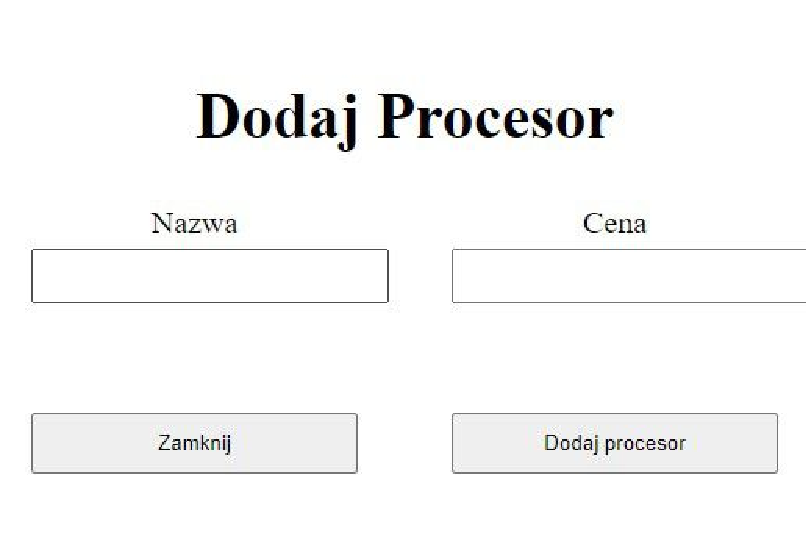
\includegraphics[width=0.35\textwidth]{rys05/view/addProc.pdf} & 
	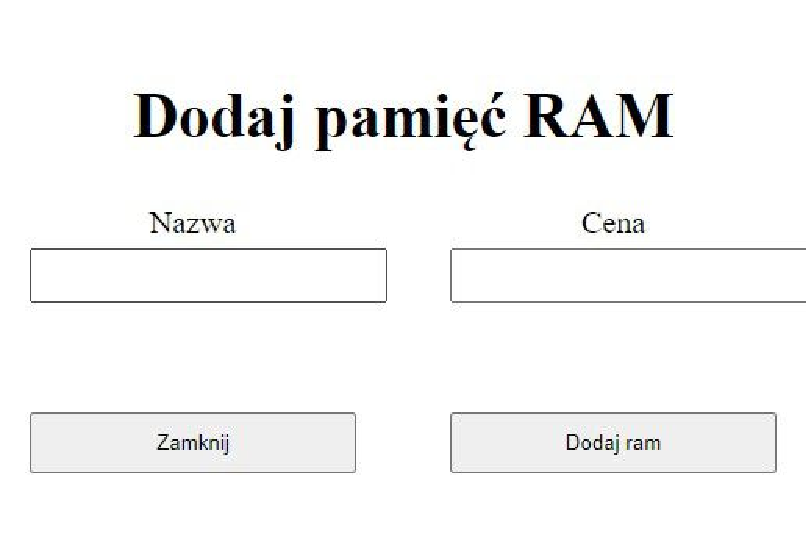
\includegraphics[width=0.35\textwidth]{rys05/view/addRam.pdf} &
	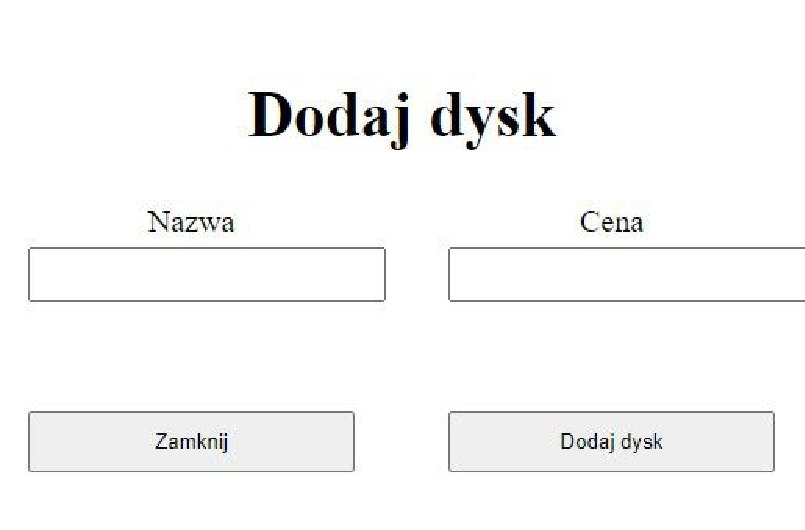
\includegraphics[width=0.35\textwidth]{rys05/view/addStorage.pdf}
	\end{tabular}
  \caption{Widok formularzy komponentów W-7, a) procesor, b) ram, c) dysk pamięci}
  \label{compforms:label}
\end{figure}

Widok W-7 \ref{compforms:label} odpowiedzialny jest za widoki formularzy komponentów. Formularze te mogą zostać wyświetlone po kliknięciu odpowiedniego przycisku na widoku W-6 \ref{components:label} lub z przycisku dostępnego na formularzu komputera(widok W-5a, W-5e, \ref{forms:label}.



